\section{Introducción}

En este trabajo se diseñó un sistema de comunicaciones digitales básico, aplicando un flujo de trabajo completo, desde la simulación en punto flotante hasta la implementación física en una FPGA. El sistema propuesto se muestra en la figura \ref{fig:esq}, que consiste en bloques generadores de PRBS, filtros transmisores, diezmador y contador de BER.

\begin{figure}[H]
    \centering
    
\includegraphics[width=0.85\linewidth]{img/esq.png}
    \caption{cap.}
    \label{fig:esq}
\end{figure}

Las características del sistema son:

\begin{itemize}
    \item \textbf{Modulación:} QPSK
    \item \textbf{Frecuencia de reloj:} 100\,MHz
    \item \textbf{Factor de sobremuestreo:} 4
    \item \textbf{Tipo de filtro:} coseno realzado de 6 baudios
    \item \textbf{Rolloff:} 0.5
    \item \textbf{Control:} Controla el funcionamiento a diferentes velocidades de los módulos del sistema.
    \item \textbf{BER:} El contador de BER realiza una etapa de inicialización cada vez que se cambia la fase de muestreo.
    \item \textbf{Seed PRBS9:} \texttt{0x1AA} (canal I) y \texttt{0x1FE} (canal Q).
\end{itemize}

\section{Objetivos}

El objetivo del trabajo es aplicar los conceptos de Python, Verilog y Aritmética de Punto Fijo aplicados
en un sistema de comunicaciones básico.

\section{Desarrollo}

\subsection{Simulación en Punto Flotante}

Se contempló todo el diseño en un simulador de punto flotante, que fue adaptado del simulador del Trabajo Práctico N°3.

Se graficó la respuesta al impulso y en frecuencia del filtro (figuras \ref{fig:float_imp} y \ref{fig:float_freq}). Luego, se graficó la convolución de este filtro con una secuencia de símbolos pseudoaleatorios (figura \ref{fig:float_conv}). Finalmente, se generaron gráficas del diagrama de ojo y constelación según la fase de muestreo (figuras \ref{fig:float_eye} y \ref{fig:float_const}).

\begin{figure}[H]
    \centering
    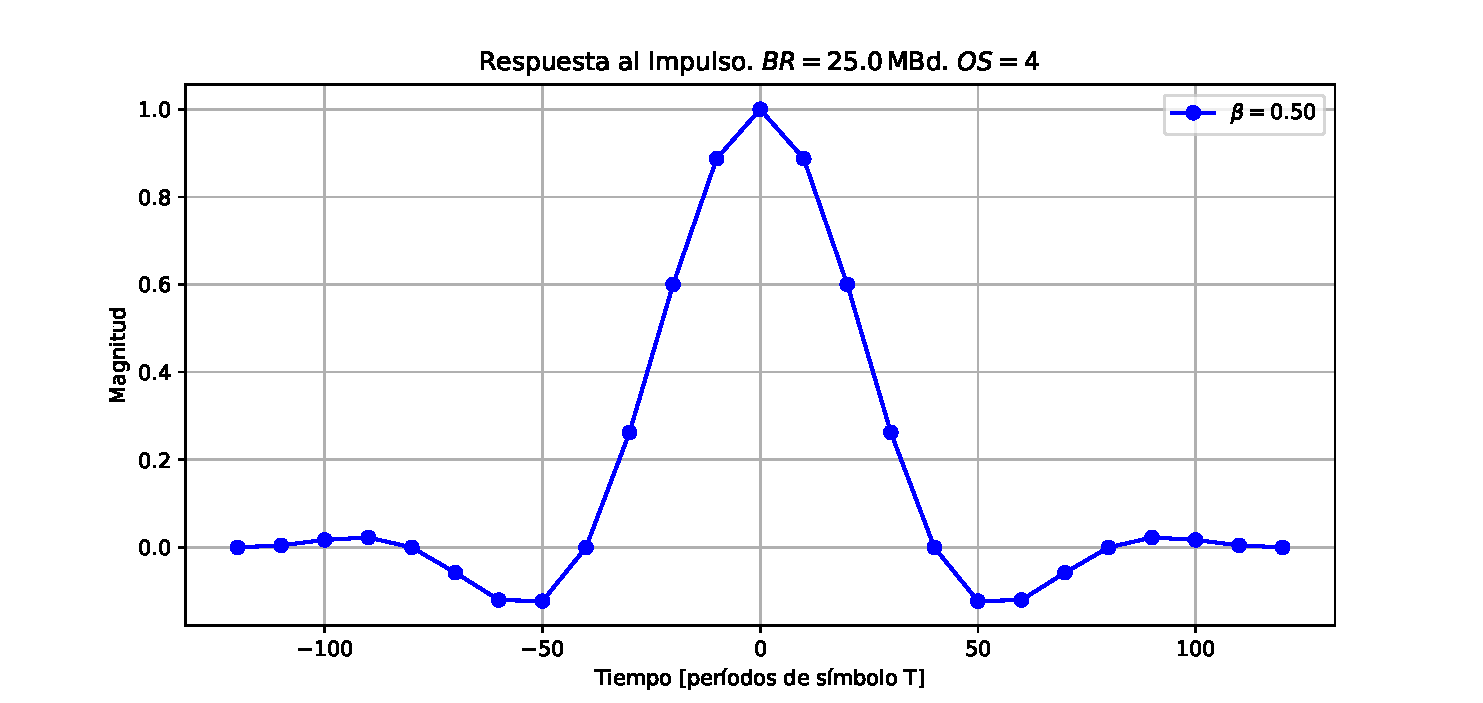
\includegraphics[width=0.85\linewidth]{img/float_imp.pdf}
    \caption{Respuesta al impulso del filtro RC a implementar.}
    \label{fig:float_imp}
\end{figure}

\begin{figure}[H]
    \centering
    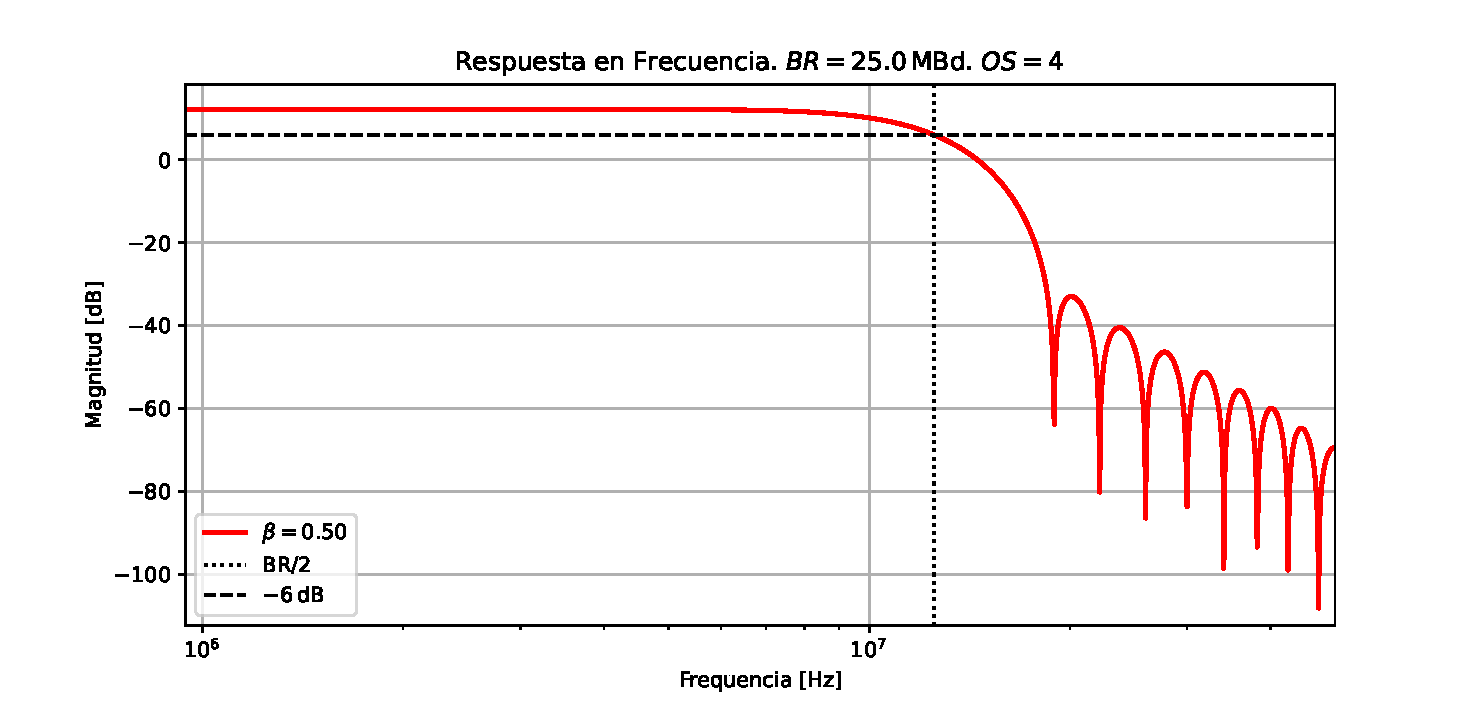
\includegraphics[width=0.85\linewidth]{img/float_freq.pdf}
    \caption{Respuesta en frecuencia del filtro RC a implementar.}
    \label{fig:float_freq}
\end{figure}

\begin{figure}[H]
    \centering
    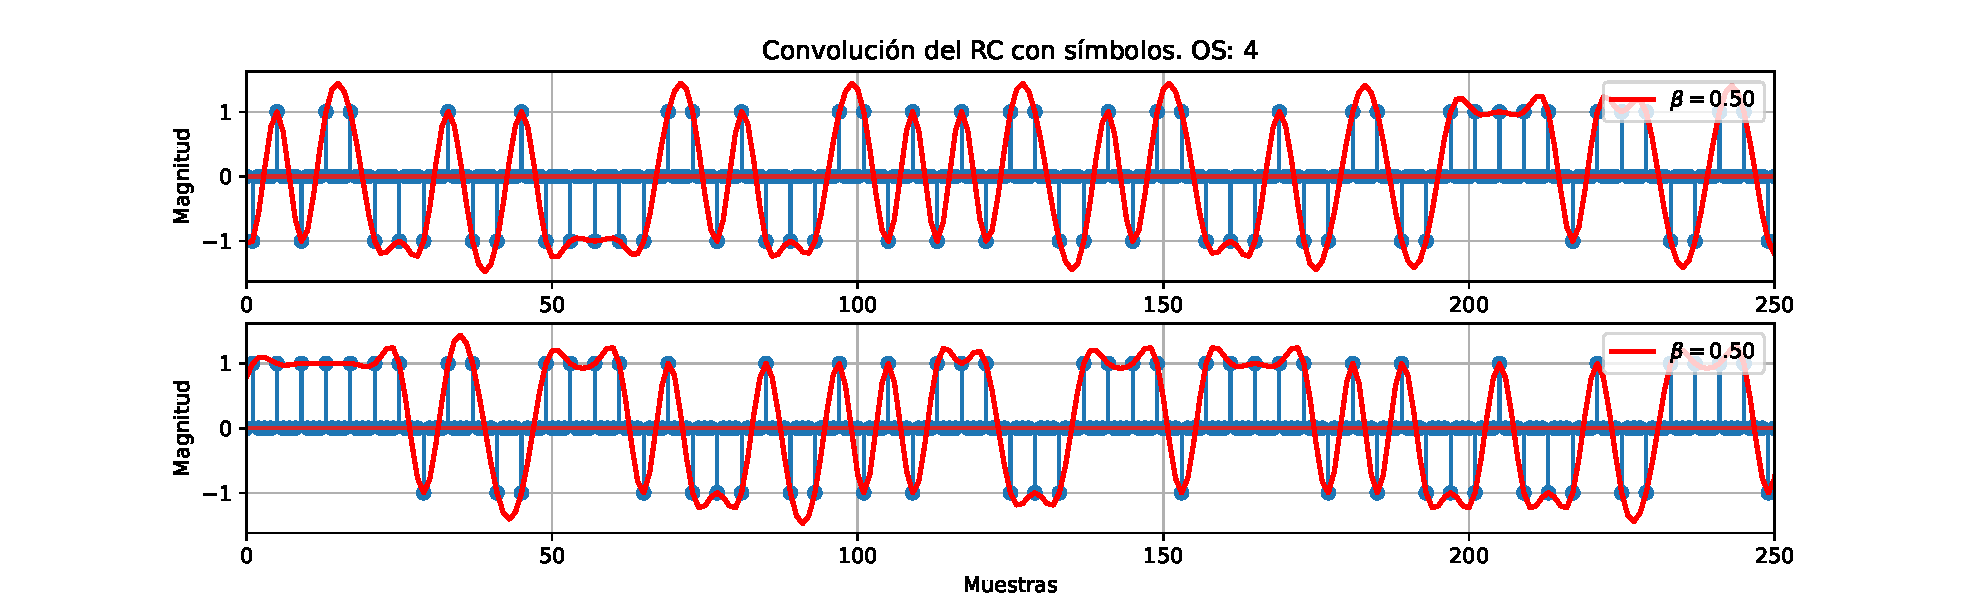
\includegraphics[width=\linewidth]{img/float_conv.pdf}
    \caption{Comparación de la salida del filtro con los símbolos generados.}
    \label{fig:float_conv}
\end{figure}

\begin{figure}[H]
    \centering
    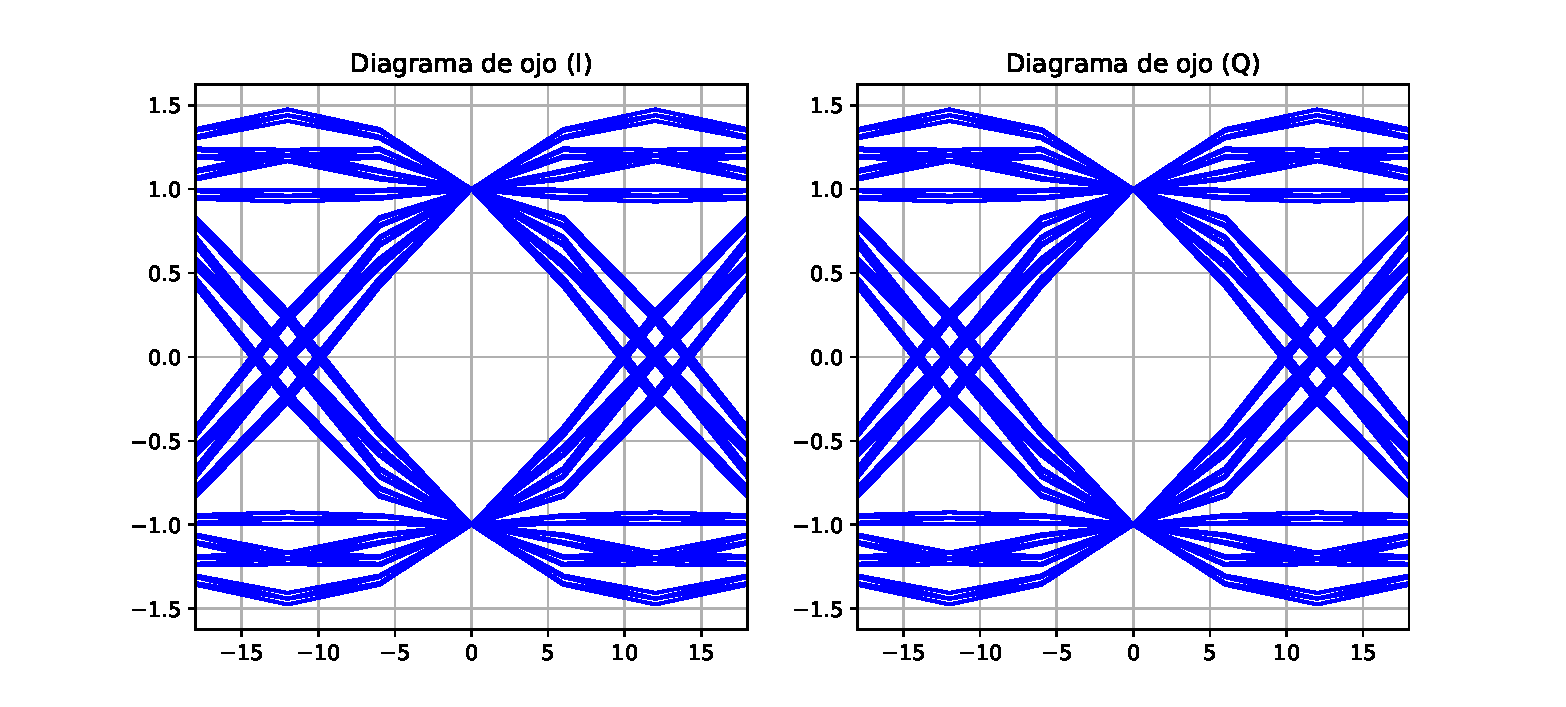
\includegraphics[width=0.9\linewidth]{img/float_eye.pdf}
    \caption{Diagrama de ojo de la salida.}
    \label{fig:float_eye}
\end{figure}

\begin{figure}[H]
    \centering
    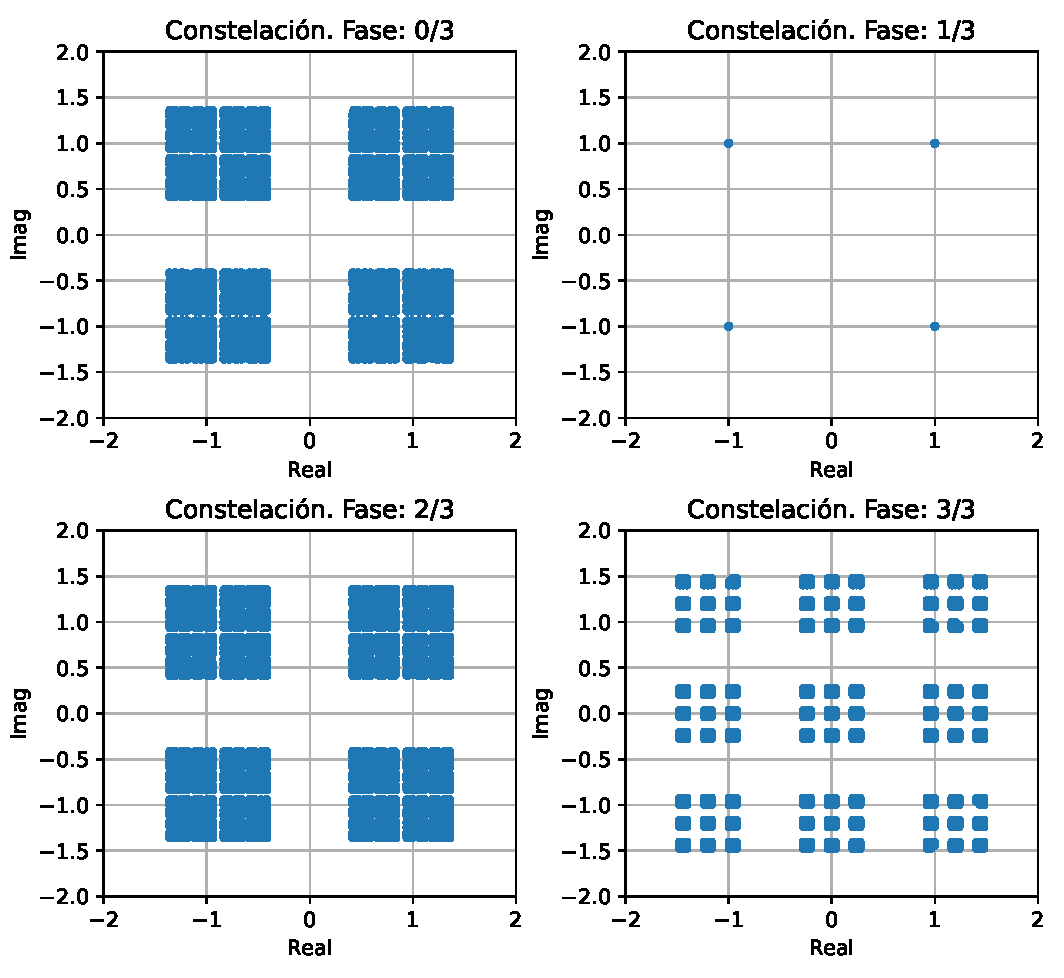
\includegraphics[width=0.9\linewidth]{img/float_const.pdf}
    \caption{Diagrama de constelación de la salida para cada fase.}
    \label{fig:float_const}
\end{figure}

La decimación se realizó para cada una de las cuatro fases posibles, descartando los primeros 100 símbolos para contar BER, ya que son parte del transitorio de la convolución con el filtro y no se llegó al estado estacionario. El resultado de BER se muestra en el cuadro \ref{tab:float_ber}, donde el único caso de errores en la decisión del símbolo es cuando la fase es igual a 3. Esto es de esperarse, ya que en la figura \ref{fig:float_const} se observa que las muestras caen dentro de la zona correcta de decisión en las fases 0, 1, y 2.

Luego de realizada la simulación, se concluyó que la cantidad de símbolos necesarios para una buena estimación de la BER es de aproximadamente 10 mil.

\begin{table}[H]
    \centering

    \begin{tabular}{lcc}
        \textbf{Fase} & \textbf{BER (I)} & \textbf{BER (Q)} \\
        \hline\hline
        0 & 0 & 0 \\
        1 & 0 & 0 \\
        2 & 0 & 0 \\
        3 & 0.18643 & 0.18623 \\
        \hline
    \end{tabular}
    \caption{BER obtenidas de la simulación.}
    \label{tab:float_ber}
\end{table}

\subsection{Simulación en Punto Fijo}



\subsection{Implementación en Verilog}



\subsection{Implementación en FPGA}



\section{Conclusión}



\appendix

\section{Scripts de Python} \label{appx:scripts}

Los scripts y RTL del trabajo se encuentran en el siguiente link: 

\noindent
\url{https://github.com/Ruben-Zuniga/Introduccion-al-Disenio-Digital/tree/main/TP4}

% \begin{equation}
%     \boxed{
%         1 = 2
%     }
% \end{equation}

% \begin{table}[H]
%     \centering
%
%     \begin{tabular}{lcc}
%         \textbf{A} & \textbf{B} & \textbf{C} \\
%         \hline\hline
%         A & B & C \\
%         A & B & C \\
%         \hline
%     \end{tabular}
%
%     \caption{cap.}
%     \label{tab:tab}
% \end{table}

% \begin{table}[H]
%     \centering
%     \begin{tblr}{
%         row{1} = {Titulo},
%         column{1} = {Titulo},
%         colspec = {Q[l] Q[c] Q[c]},
%         vlines,
%         hlines,
%         width=\linewidth
%     }
%         A & B & C \\
%         A & B & C \\
%         A & B & C \\

%     \end{tblr}
%     \caption{cap.}
%     \label{tab:tab}
% \end{table}

% \begin{figure}[H]
%     \centering
%     \includegraphics[width=0.85\linewidth]{img/sim.png}
%     \caption{cap.}
%     \label{fig:fig}
% \end{figure}

% \begin{figure}[H]
%     \centering

%     \begin{minipage}{0.48\linewidth}
%         \centering
%         \includegraphics[width=1\linewidth]{img/ondas_completo1.png}
%     \end{minipage}
%     \hfill
%     \begin{minipage}{0.48\linewidth}
%         \centering
%         \includegraphics[width=1\linewidth]{img/ondas_completo2.png}
%     \end{minipage}

%     \caption{cap.}
%     \label{fig:fig}
% \end{figure}

% \begin{figure}[H]
%     \centering

%     \begin{minipage}{\linewidth}
%         \centering
%         
\includegraphics[width=1\linewidth]{img/fulgor_logo.jpg}
%         \subcaption{cap.}
%         \label{fig:fig}
%     \end{minipage}
    
%     \begin{minipage}{\linewidth}
%         \centering
%         
\includegraphics[width=1\linewidth]{img/fulgor_logo.jpg}
%         \subcaption{cap.}
%         \label{fig:fig}
%     \end{minipage}
    
%     \begin{minipage}{\linewidth}
%         \centering
%         
\includegraphics[width=1\linewidth]{img/fulgor_logo.jpg}
%         \subcaption{cap.}
%         \label{fig:fig}
%     \end{minipage}

%     \caption{cap.}
%     \label{fig:fig}
% \end{figure}